\documentclass{../lab_class}

\usepackage{fancyhdr}
\pagestyle{fancy}
\rhead{П.\,Ю. Смирнов, 687 гр.}
\lhead{Лабораторная работа № 3.3.5, МФТИ, осень 2017}

\begin{document}

{\Large 3.3.5 -- Эффект Холла в металлах.}

\paragraph{Цель работы.}
Измерение подвижности и концентрации носителей зарядов в металлах.

В работе используются: электромагнит с источником питания, источник постоянного тока, микровольтметр, амперметры, милливеберметр, образцы из серебра и цинка.

\paragraph{Теоретическая часть.}
Ещё по полуклассической теории Бора мы знаем, что энергия электронов в атомах квантуется. Несомненно, твердое тело как макроскопическое объединение отдельных атомов имеет гораздо более сложную структуру, чем отдельный атом; тем не менее, с большой степенью точности поведение электронов в твердом теле можно описать, используя \emph{зонную модель}. В ней мы предполагаем, что каждый электрон суть <<общий>> для всех атомов данного твердого тела объект, имеющий дискретное распределение энергии (конечно, отличное от такового для отдельного атома). Вместо уровней теперь речь идёт о т.~н. зонах. Верхняя из заполненных зон -- \emph{валентная зона}; верхняя незаполненная зона -- \emph{зона подвижности}. Если все зоны заполнены, твердое тело суть диэлектрик; в противном случае оно проводник или полупроводник, в зависимости от того, как сильно заполнена зона подвижности. Во внешнем электрическом поле электроны в подвижной зоне, как ясно из данного названия, приходят в движение. Для удобства его описания обычно вводят \emph{дырки} -- квазичастицы, имеющие смысл отсутствия электрона в кристаллической решетке. Поэтому мы используем далее термин \emph{носитель заряда}, хотя де-факто есть только один вид носителя -- электрон.

\begin{wrapfigure}[12]{r}{5.5cm}
	\centering
	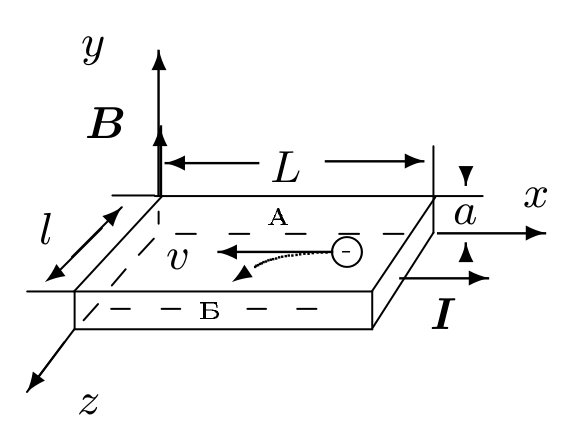
\includegraphics[width=5.5cm]{on_hall.png}
	\caption{К рассмотрению эффекта Холла}
	\label{fig:hall}
\end{wrapfigure}

Как же движутся носители заряда? Во многом похоже на механизм переноса субстанции в явлениях трения, теплопроводности и диффузии. Носитель ускоряется под действием электрического поля, проходит некоторую <<длину свободного пробега>>, врезается в какой-нибудь узел решетки, теряет скорость, и всё по новой. При этом при данных постоянных условиях (однородность вещества, постоянная температура, напряженность поля и т.~п.) можно считать, что
\begin{equation*}
	\avg{\vb{v}} = -b \vb{E},
\end{equation*}
где $b$ -- \emph{подвижность}. Пусть $n$ -- средняя концентрация носителей заряда, $e$ -- их заряд. Для плотности тока получаем тогда
\begin{equation*}
	j = n e \avg{v} = e n b E = \sigma E,
\end{equation*}
где $\sigma = e n b$ -- \emph{проводимость}. 

Мы видим, что в нашей модели\footnote{Внимательный читатель может заметить, что при <<выводе>> закона Ома и эффекта Холла мы никак не пользуемся положениями зонной теории. Бесспорно, эта теория неплохо описывает физику твердого тела качественно, однако мы не в состоянии привести ни одного количественного закона. Фактически, мы пользуемся здесь классической теорией Друде, созданной по образу и подобию кинетической теории газов (электронный газ и т.~п.).} выполняется закон Ома. С этим уже можно работать, ибо измерить проводимость -- дело простое. Заряд носителей мы знаем -- это заряд электрона, известный нам по опыту Милликена\footnote{Хотя я его не воспроизводил.}.

Ещё немного информации можно получить, если поместить образец с током в постоянное магнитное поле так, как это показано на рисунке \ref{fig:hall}. Ведь тогда на носители заряда в металле будет действовать сила Лоренца $F = e \abs{\avg{v_x}} B$, смещающая их вдоль оси $z$. Это приводит к накоплению избыточного заряда одного знака на боковых гранях А и Б пластины. Избыточный заряд, в свою очередь, создает электрическое поле, препятствующее дальнейшему накоплению заряда -- и так до тех пор, пока обе силы не уравновесят друг друга. Произойдет это, понятно, когда $E_z = \abs{\avg{v_x}} B$; в таком случае между боковыми гранями создаётся некоторое \emph{холловское напряжение} $U = -E_z l$.

\pagebreak

Замечая, что сила тока есть
\begin{equation*}
	I = n e \abs{\avg{v_x}} l a,
\end{equation*}
получаем выражение для ЭДС Холла в виде
\begin{equation}\label{eq:hall_voltage}
	U = - \frac{IB}{nea} = -R_H \frac{IB}{a},
\end{equation}
где $R_H = 1/ne$ -- \emph{постоянная Холла}. Что же мы видим? Измерение проводимости среды позволяет определить произведение $enb$, а исследование эффекта Холла -- $en$. Раз мы знаем заряд электрона, то, следовательно, можем получить из данных опытов информацию о концентрации носителей (электронов или дырок) и их подвижности, следовательно, косвенно о структуре твердого тела. Этим и займемся.

\paragraph{Экспериментальная установка.}
Суть проста -- вносим металлическую пластину в зазор электромагнита и измеряем микровольтметром ЭДС Холла. Сила тока через пластину регулируется реостатом.

\begin{figure}[H]
	\centering
	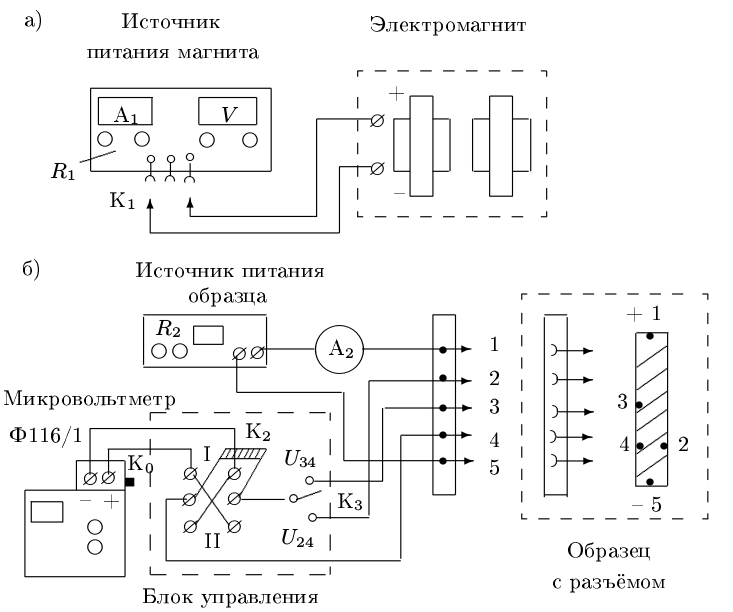
\includegraphics[width = 0.8 \textwidth]{scheme.png}
	\caption{Схема экспериментальной установки}
	\label{fig:schemet}
\end{figure}

\pagebreak

\paragraph{Измерение постоянной Холла.}
Согласно \eqref{eq:hall_voltage}, постоянная Холла суть функция двух параметров -- силы тока и магнитного поля. Поэтому для её нахождения мы сначала проведём несколько серий измерений для построения графика функции $U_H = f(B)$ при разных значениях силы тока $I$ через образец, а затем по полученным угловым коэффициентам $k$ построим искомый график $k = f(I)$, из которого и определяется постоянная Холла. 

Прежде, однако, выполним калибровку электромагнита ради известной зависимости $B = f(I_m)$ (где $I_m$ -- ток через электромагнит):

\begin{figure}[H]
	\centering
	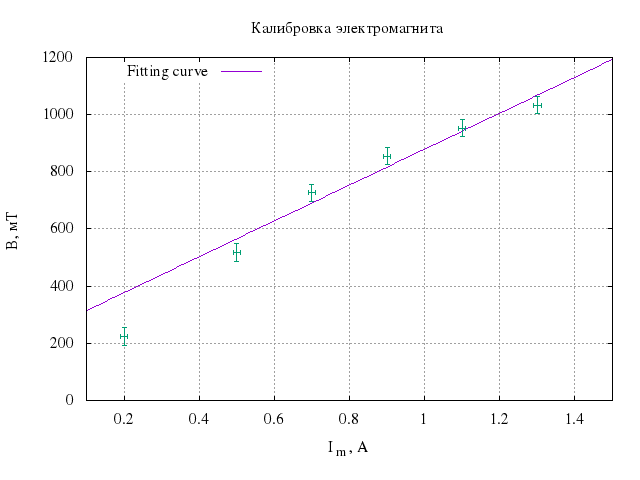
\includegraphics[width = 0.65 \textwidth]{electromagnet.png}
	\caption{Калибровка электромагнита}
\end{figure}

Будем использовать пластину серебра. Для токов $I = 0.2 - 1.3 \ \A$ имеем следующие линейные зависимости:
\begin{figure}[H]
	\centering
	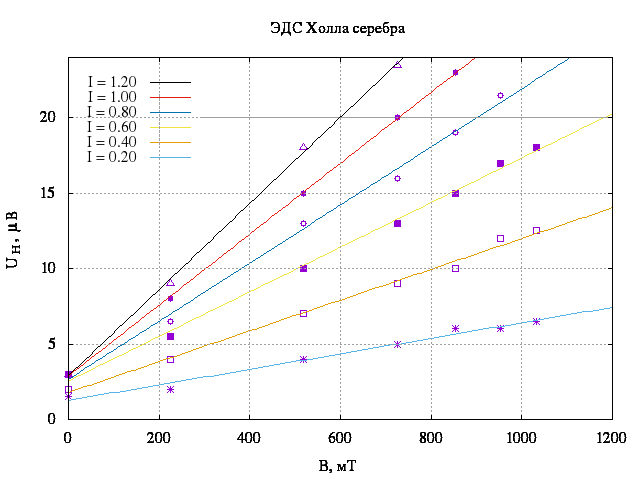
\includegraphics[width = 0.65 \textwidth]{silver.png}
	\caption{Зависимость ЭДС Холла пластины из серебра от напряженности магнитного поля при разных значениях силы тока через пластину}
\end{figure}

Отсюда получаем зависимость углового коэффициента $k = f(I)$:
\begin{figure}[H]
	\centering
	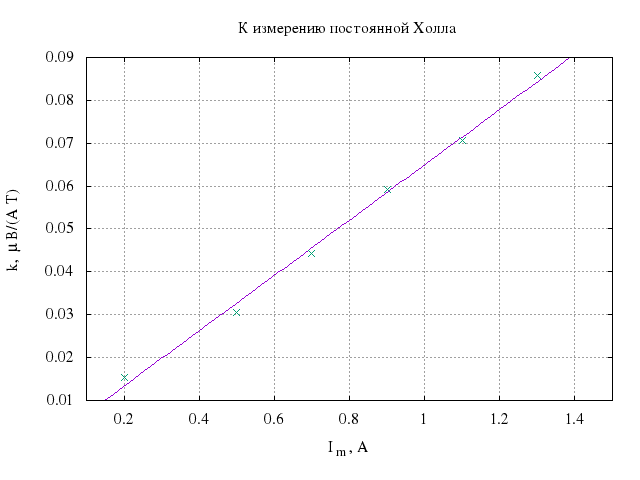
\includegraphics[width = 0.65 \textwidth]{hall_constant.png}
	\caption{К определению постоянной Холла серебра}
\end{figure}

Получаем коэффициент $k \simeq (6.4 \pm 0.2) \times 10^{-7} \ \V / \A \cdot \T$. Толщина серебряной пластины $a = 0.09 \ \sm \m$; отсюда по формуле $\eqref{eq:hall_voltage}$ имеем
\begin{gather*}
	R_H^{\text{Ag}} \simeq (-5.7 \pm 0.2) \times 10^{-11} \ \V \cdot \m / \A \cdot \T.
\end{gather*}
Заметим здесь сразу, что нужно быть осторожным при попытке сравнения с табличными значениями, т.~к. реальное значение постоянной Холла зависит от температуры пластины, её геометрии и даже магнитного поля. Например, в учебном методическом пособии университета Теннесси (США) приводится значение $\approx 8$, совпадающее по порядку с нашим. Думаю, это успех.

Всего одна серия аналогичных измерений была проведена также для пластины цинка при токе $I = 1.2 \ \A$:
\begin{figure}[H]
	\centering
	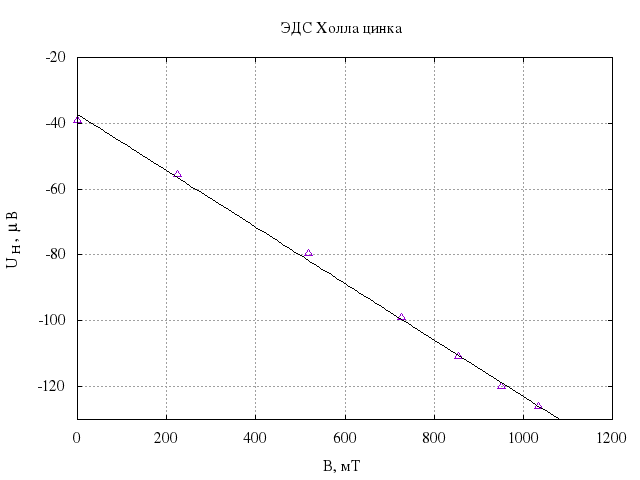
\includegraphics[width = 0.6 \textwidth]{zinc.png}
	\caption{К определению постоянной Холла цинка}
\end{figure}

\pagebreak

Толщина пластины цинка $a = 0.12 \ \sm \m$; отсюда имеем $k \simeq (-8.5 \pm 0.1) \times 10^{-7} \ \V / \A \cdot \T$ и постоянную Холла
\begin{gather*}
	R_H^{\text{Zn}} \simeq (1.02 \pm 0.15) \times 10^{-10} \ \V \cdot \m / \A \cdot \T.
\end{gather*}
Удивительно, тоже весьма похоже на табличное значение $1.04$! Важный момент, требующий внимания -- знак постоянной Холла серебра и цинка отличается. Это говорит о том, что в первом случае носители заряда суть электроны, во втором -- дырки.

\paragraph{Носители заряда и их подвижность.}
Теперь мы можем непосредственно легко найти важные параметры металла -- концентрацию носителей заряда и их подвижность. Выше мы уже определили постоянную Холла и даже сразу смогли указать тип носителей. Теперь элементарно вычислим проводимость материала образца:
\begin{equation*}
	\sigma = \frac{I L}{U a l}.
\end{equation*}
Для пластины серебра $L = 15 \ \sm \m$, $l = 11 \ \sm \m$; для цинка -- $L = 3.5 \ \sm \m$, $l = 10.5 \ \sm \m$. Толщина пластины указана ранее. Измерим падение напряжения на пластине при пропускании через неё тока $I = 1 \ \A$: $U_{\text{Ag}} = 28.05 \ \sm \V$, $U_{\text{Zn}} = 26.17 \ \sm \V$. Отсюда имеем
\begin{gather*}
	\sigma_{Zn} = 1.06 \times 10^7 (\Ohm \cdot \m)^{-1}, \\
	\sigma_{Ag} = 5 \times 10^7 \ (\Ohm \cdot \m)^{-1}.
\end{gather*}

Концентрация носителей заряда есть $n = 1/R_He$:
\begin{gather*}
	n_{\text{Ag}} = 1.1 \times 10^29,\\
	n_{\text{Zn}} = 6.1 \times 10^28.
\end{gather*}

Тогда легко получаем подвижность $b = \sigma R_H$:
\begin{gather*}
	b_{\text{Ag}} = 2.8 \times 10^{-3} \ \m^2 / (\V \cdot \s), \\
	b_{\text{Zn}} = 5.1 \times 10^{-3} \ \m^2 / (\V \cdot \s).	
\end{gather*}
Табличные данные есть $5.6$ и $1.75$ соответственно.

\paragraph{Выводы.}
Предложенная схема эксперимента при всей своей простоте дает результат точности достаточной, чтобы оценить порядок величин, характеризующих природу материала -- концентрацию носителей заряда и их подвижность в кристаллической решетке. Заметим также, что мы попутно сразу определяем тип носителей заряда и можем легко (в рамках модели Друде) оценить даже длину свободного пробега и среднее время между столкновениями носителей\footnote{В подробности, однако, не будем пока углубляться.}. 

\end{document}